\documentclass[11pt, aspectratio=169]{beamer}
%\documentclass[11pt,handout]{beamer}
\usepackage[T1]{fontenc}
\usepackage[utf8]{inputenc}
\usepackage{textcomp}
\usepackage{float, afterpage, rotating, graphicx}
\usepackage{epstopdf}
\usepackage{longtable, booktabs, tabularx}
\usepackage{fancyvrb, moreverb, relsize}
\usepackage{eurosym, calc}
\usepackage{amsmath, amssymb, amsfonts, amsthm, bm}
\usepackage[
    natbib=true,
    bibencoding=inputenc,
    bibstyle=authoryear-ibid,
    citestyle=authoryear-comp,
    maxcitenames=3,
    maxbibnames=10,
    useprefix=false,
    sortcites=true,
    backend=biber
]{biblatex}
\AtBeginDocument{\toggletrue{blx@useprefix}}
\AtBeginBibliography{\togglefalse{blx@useprefix}}
\setlength{\bibitemsep}{1.5ex}
\addbibresource{refs.bib}

\hypersetup{colorlinks=true, linkcolor=black, anchorcolor=black, citecolor=black, filecolor=black, menucolor=black, runcolor=black, urlcolor=black}

\setbeamertemplate{footline}[frame number]
\setbeamertemplate{navigation symbols}{}
\setbeamertemplate{frametitle}{\centering\vspace{1ex}\insertframetitle\par}


\begin{document}

\title{Elevating Trust by increasing Instruction hours-German G8 Reform }

\author[Adrija Roy]
{
{\bf Adrija Roy}\\
{\small University of Bonn}\\[1ex]
}


\begin{frame}
    \titlepage
    \note{~}
\end{frame}


\begin{frame}[t]
    \frametitle{Contents}
    \begin{itemize}
        \item<+-> This presentation only has the graphs used in the actual paper.
        \item<+->  Template used- \citet{GaudeckerEconProjectTemplates}
    \end{itemize}   
    \note{~}
\end{frame}



\begin{frame}[t]
    \begin{figure}[H]

        \centering
        \includegraphics[width=0.5\textwidth]{../bld/python/figures/descriptive_stats}

        \caption{\emph{Python:} Descriptive statistics by treatment status}
        \label{fig:descriptive_stats_pres}

    \end{figure}
\end{frame}

\begin{frame}[t]
    \begin{figure}[H]

        \centering
        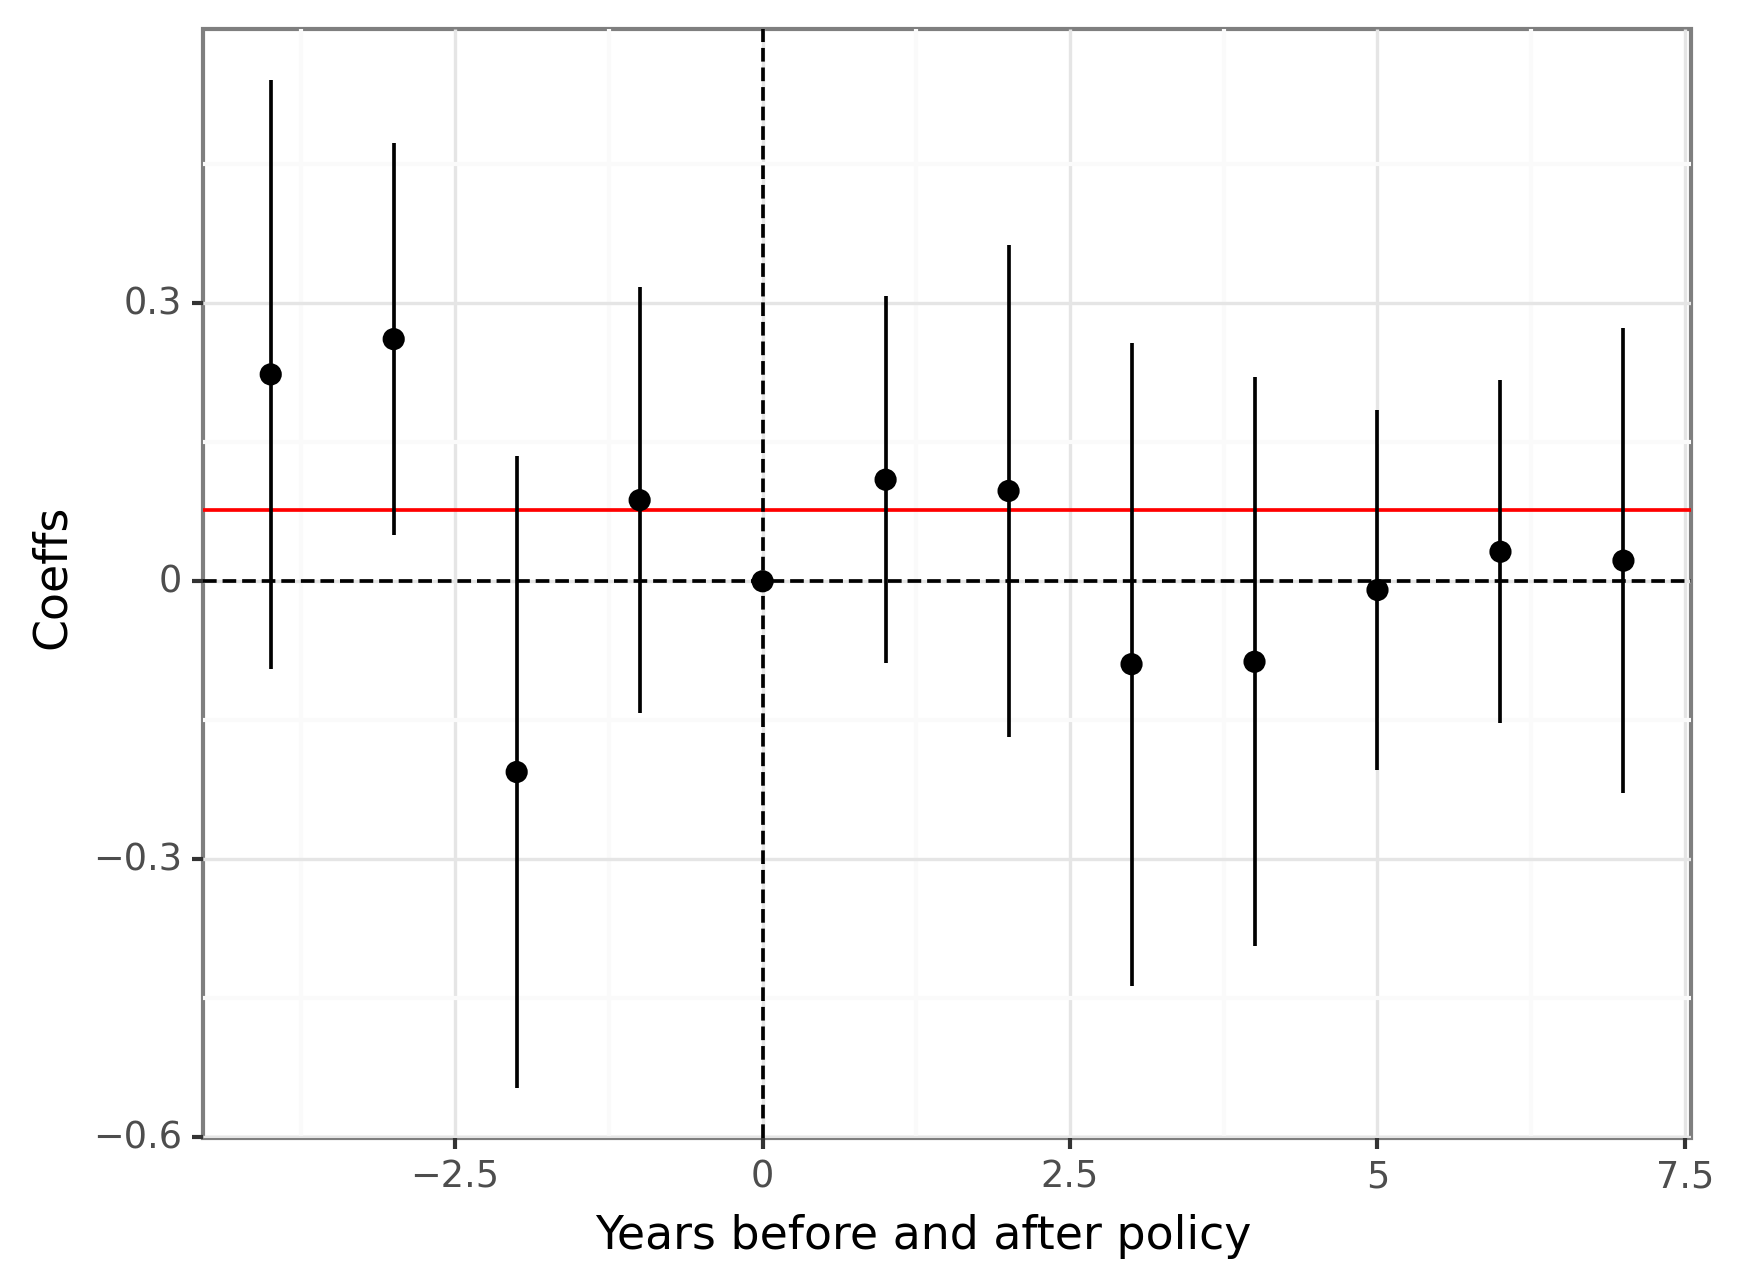
\includegraphics[width=0.5\textwidth]{../bld/python/figures/event_study_gym}

        \caption{\emph{Python:} Event study graph with 4 lags and 7 leads}
        \label{fig:event_study_pres}

    \end{figure}
\end{frame}



% Print black screen only in presentation mode for finishing up.
\mode<beamer> {
    \beamersetaveragebackground{black}
    \begin{frame}
        \frametitle{}
    \end{frame}

    \beamersetaveragebackground{white}
}

\begin{frame}[allowframebreaks]
    \frametitle{References}
    \renewcommand{\bibfont}{\normalfont\footnotesize}
    \printbibliography
\end{frame}

\end{document}
